\documentclass[final, t]{beamer} % beamer 3.10: do NOT use option hyperref={pdfpagelabels=false} !
\usetheme{ASblue} 

\usepackage[polish]{babel}
\usepackage{wrapfig}

\usepackage[utf8]{inputenc}
\usepackage[OT4]{polski}
\usepackage{amsmath,amsthm, amssymb, latexsym}

\usepackage[orientation=landscape,size=a0,scale=1.4]{beamerposter}                       % e.g. for DIN-A0 poster
\title{Odzyskiwanie parametrów kinetycznych rozplatania kinazy tytyny 1TKI z symulacji dynamiki molekularnej}
\author{\textit{Mateusz Najsztub}\\ Opiekun pracy:  prof. dr hab. Andrzej Molski}
\institute{Zakład Chemii Fizycznej Uniwersytetu im. Adama Mickiewicza w Poznaniu}
\date{}
  
  
  \begin{document}
  \begin{frame}{} 
 \begin{columns}[T]
  \begin{column} {.4\textwidth}
    \begin{block}{Wprowadzenie}
    \centering
    \begin{minipage}{0.97\textwidth}

    Wraz z rozwojem techniki aparaturowej pojawiły się nowe narzędzia badania procesów molekularnych na poziomie pojedynczej cząsteczki. Jednym z takich narzędzi jest mikroskop sił atomowych (AFM). Celem pracy było zbadanie możliwości ekstrapolacji danych eksperymentalnych z wyników symulacji rozplatania kinazy tytyny 1TKI. W tym celu dopasowano krzywą teoretyczną zależności maksymalnych sił rozplatania od prędkości rozplatania do wartości uzyskanych z symulacji programem \textbf{Gromacs} [1] na klastrze obliczeniowym zbudowanym na Zakładzie Chemii Fizycznej.
    \end{minipage}
        \end{block}
        \begin{block}{Schemat eksperymentu}
        \centering
         \begin{minipage}{0.97\textwidth}

        \includegraphics[width=0.48\linewidth]{afm1.png}
        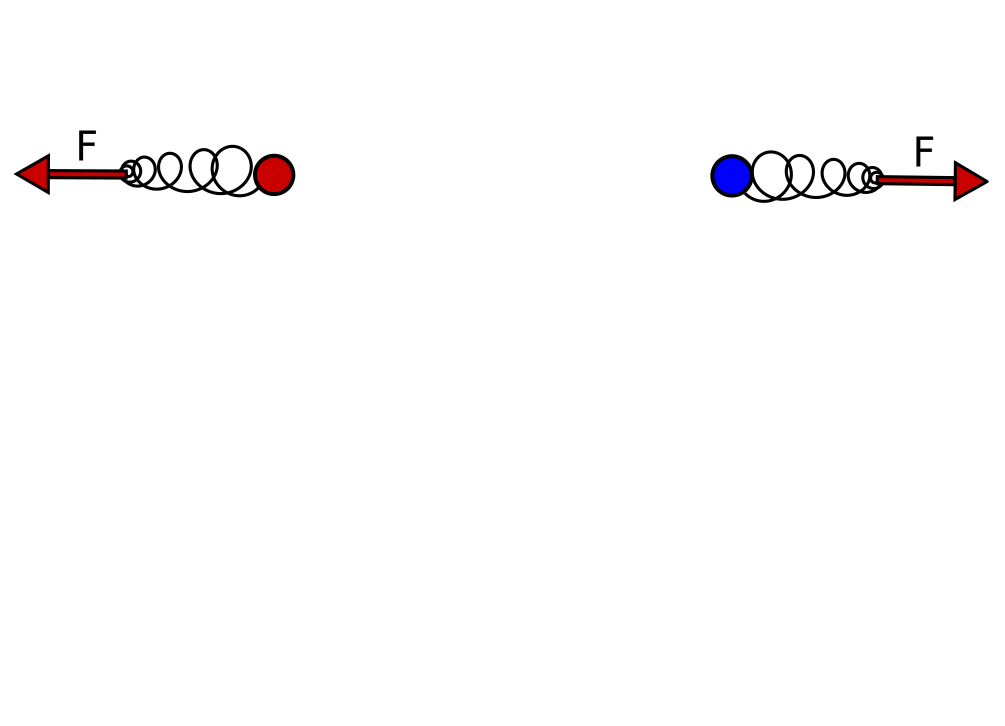
\includegraphics[width=0.48\linewidth]{mol.png}\\

        (a) Rysunek ideowy przedstawiający aparaturę do eksperymentów AFM. Podczas rozciągania cząsteczki mierzona jest siła aż do jej rozplecenia. (b) Wizualizacja kinazy tytyny, 1TKI użytej w obliczeniach. Symulacja polega na odsuwaniu ze stała szybkością wirtualnej sprężyny o stałej sprężystości $k$ przytwierdzonej do N-końca i C-końca białka.
        \end{minipage}
        
        \end{block}
        \begin{block}{Metodologia}
        \centering
         \begin{minipage}{0.97\textwidth}
       \includegraphics[width=0.32\linewidth]{rmsd.pdf}
        \includegraphics[width=0.66\linewidth]{plot.png}\\
       (a) Wykres RMSD (Root-Mean-Square Deviation) pokazujący odchylenie struktury białka podczas symulacji w czasie od struktury wyjściowej. Równowagowanie przeprowadzano przez 7.5 ns w pudle o wymiarach 7.8 x 8.4 x 18.6 nm przy około 120000 atomach. Rysunek (b) przedstawia wizualizację układu z białkiem, zaznaczonymi atomami tlenu od cząsteczek wody oraz jonami Na$^{+}$ oraz Cl$^{-}$.
        \end{minipage}
        \end{block}
       
    \end{column}
    \begin{column} {.58\textwidth}
        \begin{block}{Przykładowe trajektorie rozciągania}\vspace{10mm}
        \centering
         \begin{minipage}{0.97\textwidth}
       \includegraphics[width=0.49\linewidth]{pull.png}
        \includegraphics[width=0.49\linewidth]{pull2.png}\\
        Porównanie dwóch trajektorii dla prędkości rozciągania 0.8 i 5 nm/ns dla N i C-końca (zielony i niebieski). Maksymalne siły rozplatania były brane jako maksymalne siły na wygładzonym wykresie siły od rozciągnięcia (linia ciągła).
        \end{minipage}\vspace{10mm}
        \end{block}
        
          \begin{block}{Analiza danych}\vspace{10mm}
          \centering
         \begin{minipage}{0.97\textwidth}

       \includegraphics[width=\linewidth]{anal3.png}

Do uzyskanych sił zerwania dopasowano metodą najmniejszych kwadratów krzywą teoretyczną z modelu Hummer-Szabo metodą opisaną w publikacji [2]. Dopasowanymi parametrami były stała zerwania $k_{0}$, stała sprężystości białka $k_{s}$ oraz długość, przy której białko ulega rozpleceniu $x_{b}$. Krzywą dopasowano do samych wyników symulacji (a) oraz do wyników symulacji z wynikiem eksperymentu dla niskiej szybkości rozciągania, 50 pN przy 1$\mu$m/s (b). Tę samą metodę zastosowano dla wyników z publikacji [3] (c i d).
\vfill
\end{minipage}\vspace{10mm}
        \end{block}

    \begin{block}{Wnioski}
    \vspace{10mm}
    \centering
         \begin{minipage}{0.97\textwidth}
    \begin{itemize}
    \item Dane eksperymentalne nie zgadzają się z symulacjami. Przedstawiona metoda dopasowania jest bardzo czuła na błędy statystyczne powstałe w wyniku ograniczonej liczby powtórzeń symulacji i daje mocno rozbieżne wyniki. 
    \item Rozwiązaniem powyższego problemu są wielokrotne powtórzenia symulacji dla większych szybkości oraz symulacje dla większego zakresu prędkości. Obliczenia te są jednak czasochłonne.

    \item Wydajność klastra zbudowanego na komputerach wielordzeniowych jest ograniczona przez sieć 1 Gbps, która jest o wiele wolniejsza w porównaniu do komunikacji pomiędzy rdzeniami procesorów znajdujących się na jednej płycie głównej.

    \end{itemize}
    \end{minipage}
    \vspace{10mm}
    \end{block}

    \end{column}
    \end{columns}
    \begin{block}{Literatura}
      \centering
         \begin{minipage}{0.97\textwidth}   
          [1] B. Hess et al.  Gromacs user manual version 4.5. www.gromacs.org
         
    [2] K. Schulten et al. Discovery Through the Computational Microscope. Structure, 17(10):1295 -- 1306, 2009

    
    [3] H. Grubmüller et al. Mechanically induced titin kinase activation studied by forceprobe molecular dynamics simulations. Biophysical Journal, 88(2):790 -- 804, 2005.

    


    \end{minipage}
    \end{block}
    \vfill
  \end{frame}
  \end{document}
  